
\section{Thin Strip Graphs}
\label{sec:thin}


$c$-strip graphs are unit disk graphs such that the centers of the disks belong to
$\{(x,y) : -\infty < x < \infty, 0 < y \leq c\}$. The class is denoted by SG($c$). We
have SG(0) = UIG and SG($\infty$) = UDG. \cite{hayashiThinStripGraphs2017}

\begin{defn}
  Thin strip graphs are defined as TSG $= \bigcap_{c > 0}$ SG($c$).
\end{defn}

\begin{remark}
  SG($0$) $\neq$ TSG. We can construct a $K_{1,3}$ such that we have 3 vertices with the coordinates
  $(1,0)$, $(0,0)$, $(1,0)$ and a last one $(0,\varepsilon)$ with $\varepsilon > 0$ as seen in Figure \ref{fig:thinK13}.
\end{remark}


% Figure about the K_1,3 construction
\begin{figure}
\centering

\begin{scaletikzpicturetowidth}{\textwidth}
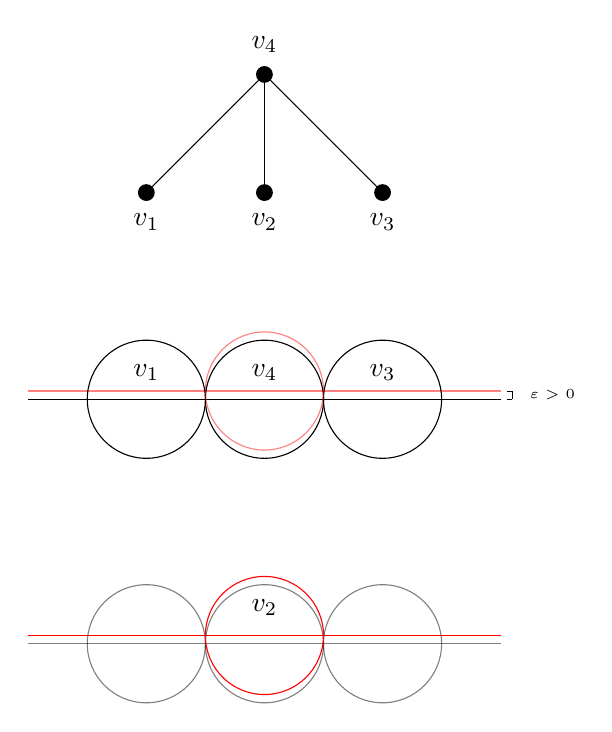
\begin{tikzpicture}[scale=1.5]

\draw (-2,0) -- (2,0);
\draw[red ,opacity = 0.5] (-2,0.07) -- (2,0.07);
\draw  (-1,0) circle [radius=0.5];
\draw[color=black] (-1,0.2265) node {$v_1$};
\draw  (0,0) circle [radius=0.5];
\draw[color=black] (0,0.2265) node {$v_4$};
\draw  (1,0) circle [radius=0.5];
\draw[color=black] (1,0.2265) node {$v_3$};

\draw[red, opacity = 0.5] (0,0.07) circle [radius=0.5];

\draw[color=black] (2.4386,0.0367) node {\tiny $\varepsilon > 0$};

% lines to describe distance (epsilon)
\draw[very thin] (2.1,0.07) -- (2.1,0);
\draw[very thin] (2.05,0.07) -- (2.1,0.07);
\draw[very thin] (2.05,0) -- (2.1,0);

\draw[opacity = 0.5] (-2,-2.07) -- (2,-2.07);
\draw[red] (-2,-2) -- (2,-2);
\draw[opacity = 0.5]  (0,-2.07) circle [radius=0.5];
\draw[opacity = 0.5]  (1,-2.07) circle [radius=0.5];
\draw[opacity = 0.5]  (-1,-2.07) circle [radius=0.5];
\draw[red] (0,-2) circle [radius=0.5];
\draw[color=black] (0,-1.765) node {$v_2$};

\node[draw,circle,inner sep=2pt,fill,label distance=1cm] (v1) at (0,2.75) {};
\draw[color=black] (0,3) node {$v_4$};
\node[draw,circle,inner sep=2pt,fill,label distance=1cm] (v3) at (0,1.75) {};
\draw[color=black] (0,1.5) node {$v_2$};
\node[draw,circle,inner sep=2pt,fill,label distance=1cm] (v2) at (-1,1.75) {};
\draw[color=black] (1,1.5) node {$v_3$};
\node[draw,circle,inner sep=2pt,fill,label distance=1cm] (v4) at (1,1.75) {};
\draw[color=black] (-1,1.5) node {$v_1$};
\draw  (v1) edge (v2);
\draw  (v1) edge (v3);
\draw  (v1) edge (v4);
\end{tikzpicture}
\end{scaletikzpicturetowidth}

\caption{A construction of $K_{1,3}$ with a disk realization, being this graph a TSG.}
\label{fig:thinK13}
\end{figure}

It has been proven that MUIG $\subsetneq$ TSG.\\


Denote that there's not constant $t$ such that SG($t$) = TSG.\\

Unfettered unit interval graphs = UUIG\\

MUIG $\subsetneq$ TSG $\subsetneq$ UUIG\\

UUIG $\subseteq$ co-comparability graphs (to prove).
\paragraph{Proof} Let's have a relation of non-increasing order $\leq$ between the left
endpoints of each interval $v$ ($l(v)$). This relation will (nope, find another proof...).


\subsection{Open questions about Thin Strip Graphs}
In this section we state the problems that are being studied for the thesis.

\paragraph{Forbidden subgraphs of Thin Strip Graphs}
  We've proven that MUIG $\subsetneq$ TSG $\subsetneq$ UUIG. Knowing the\\
  (Why $F_k$ is a co-comparability unit disk graph?)

\paragraph{Complexity class for TSG recognition}
  We've shown in section \ref{sec:complex} that some intersection
  geometric problems are in $\exists \mathbb{R}$ (unit disk graph
  recognition problem or the stretchability problem) and we'd like to
  know if TSG recognition or even SG($c$) recognition is in NP knowing
  that TSG $\subseteq$ UDG $\cap$ UUIG.

\paragraph{Complexity class of graph problems applied in TSG}
  We've shown in section \ref{sec:complex} that CLIQUE is in $\mathcal{P}$ for
  unit disk graphs. Knowing that TSG $\subseteq$ UDG $\cap$ UUIG we know that CLIQUE
  is also polynomial for TSG. The question is, is there any problem that for the superclasses
  UUIG (and also co-comparability graphs) and UDG such that their complexity is reduced
  when applied to TSGs?
